\chapter{Aplicación Web}
\label{cap:aplicacionWeb}

La aplicación web se ha creado con el objetivo de proporcionar una interfaz web atractiva y manejable tanto para los terapeutas como para sus pacientes. Ahora bien, el chatbot es la esencia de este TFG y, por tanto, es la herramienta principal que se desarrolla en la página web. El chatbot se ha pensado para ser utilizado por los pacientes. La aplicación web permite probar el chatbot de forma mucho más manejable y visible que desde un terminal del entorno de desarrollo. Además, se ha querido añadir más funcionalidades para los terapeutas que, podrán acceder a los recuerdos de sus pacientes de forma sencilla y visual. En este capítulo se explicarán los pasos que se han seguido para desarrollar la página web desde el principio con un prototipo inicial a mano alzada hasta el final con una aplicación web funcional y con numerables vistas. 


\section{Prototipo inicial}

Al comienzo de este trabajo, había que ver qué dirección se iba a seguir y por ello, se plantearon diferentes propuestas para luego ser guiada por la más adecuada. Una de las ideas iniciales que se propusieron fue la de crear una aplicación web. Se realizó un esbozo sobre lo que se creía que iba a necesitar un chatbot como aplicación para estar completo. Este prototipo a mano alzada está dividido en dos partes. Por un lado, están las funcionalidades pensadas para el uso del terapeuta, que podrá programar las sesiones que quiere hacer personalmente con el paciente (ver Figuras \ref{fig:diseñoinicialappterapeuta1}, \ref{fig:diseñoinicialappterapeuta2}, \ref{fig:diseñoinicialappterapeuta3}, \ref{fig:diseñoinicialappterapeuta4}, \ref{fig:diseñoinicialappterapeuta5}). Por otro lado, las funcionalidades que están pensadas para el paciente con demencia (ver Figura \ref{fig:diseñoinicialappusuario}) y que hará uso del chatbot en sí. Es importante aclarar que no se planteó como sustituto de las sesiones que tienen los terapeutas con sus  pacientes y que las funcionalidades que tiene disponibles en la aplicación son para ayudarle a programar esas sesiones. El chatbot debe estar accesible desde la cuenta de un paciente para facilitar la tarea del terapeuta en la recopilación de sus recuerdos.

Para el usuario con demencia el prototipo es muy sencillo, tiene 2 funcionalidades básicas propias (ver Figura \ref{fig:diseñoinicialappusuario}):

\begin{figure}[h]
	\centering
	\includegraphics[scale=1.0]{Imagenes/Vectorial/diseño app tfg 2}
	\caption{Prototipo inicial de la aplicación para el usuario con demencia}
	\label{fig:diseñoinicialappusuario}
\end{figure}

\begin{itemize}
	\item Chatbot: La pestaña de terapia lleva al usuario al chat donde se le hará preguntas sobre su vida para recabar el máximo número de recuerdos. El chatbot es un complemento aparte que ayuda al terapeuta a recoger la información del usuario pero que no sustituye las sesiones habituales paciente-terapeuta.
	\item Historia de vida: Los recuerdos recabados se guardan en la aplicación y el usuario puede consultarlos divididos por etapas de la vida (infancia, adolescencia, etapa adulta, etc.). Esto sería parte de la terapia ocupacional basada en reminiscencia y un paso previo para construir el libro de vida del usuario. El usuario puede revisitar sus recuerdos a través de la aplicación y esto puede ayudar en el retraso del deterioro cognitivo.
\end{itemize}

En cuanto a las vistas del terapeuta, tendrá muchas más funcionalidades disponibles:

\begin{figure}[h]
	\centering
	\includegraphics[scale=0.1]{Imagenes/Vectorial/diseño app tfg 1-1}
	\caption{Prototipo inicial de la aplicación para el terapeuta: Consultar los pacientes registrados}
	\label{fig:diseñoinicialappterapeuta1}
\end{figure}


\begin{itemize}
	\item Pacientes: Se muestra una lista de los usuarios (pacientes) que tiene el terapeuta asignados y que están registrados en la aplicación (ver Figura \ref{fig:diseñoinicialappterapeuta1}). 
\end{itemize}

\begin{figure}[h]
	\centering
	\includegraphics[scale=0.1]{Imagenes/Vectorial/diseño app tfg 1-2}
	\caption{Prototipo inicial de la aplicación para el terapeuta: Consultar los datos de un paciente 1}
	\label{fig:diseñoinicialappterapeuta2}
\end{figure}


\begin{itemize}
	\item Datos personales del paciente: Los datos personales y clínicos del paciente estarán disponibles para que el terapeuta los consulte cuando quiera (ver Figura \ref{fig:diseñoinicialappterapeuta2}).
	\item Terapias del paciente: Se muestran las terapias que se han creado para ese paciente, tanto las que se programaron para fechas pasadas como las que ocurrirán próximamente (ver Figura \ref{fig:diseñoinicialappterapeuta2}). El terapeuta es el que crea estas terapias para sus futuras sesiones con el paciente, las terapias pasadas son las sesiones que se han finalizado y las próximas son las que están pendientes por hacer.
\end{itemize}

\begin{figure}[h]
	\centering
	\includegraphics[scale=0.1]{Imagenes/Vectorial/diseño app tfg 1-3}
	\caption{Prototipo inicial de la aplicación para el terapeuta: Consultar los datos de un paciente 2}
	\label{fig:diseñoinicialappterapeuta3}
\end{figure}


\begin{itemize}
	\item Historia de vida del paciente: Los recuerdos recabados en las sesiones terapéuticas se guardan en la aplicación y el terapeuta puede consultarlos divididos por etapas de la vida (infancia, adolescencia, etapa adulta, etc.) igual que podía hacer el usuario (ver Figura \ref{fig:diseñoinicialappterapeuta3}). El objetivo de que el terapeuta pueda consultarlos es para revisar que se han grabado los recuerdos correctamente y para comprobar que son precisos y coherentes. En cualquier caso, el terapeuta podrá editar o borrar los recuerdos que crea incompletos o incorrectos y podrá también añadir recuerdos que haya conseguido de alguna otra forma. En caso de que algún recuerdo esté mal clasificado en la etapa de la vida en que ocurrió, también se podría mover a su sitio correcto.
\end{itemize}

\begin{figure}[h]
	\centering
	\includegraphics[scale=0.08]{Imagenes/Vectorial/diseño app tfg 1-4}
	\caption{Prototipo inicial de la aplicación para el terapeuta: Crear y consultar las terapias creadas}
	\label{fig:diseñoinicialappterapeuta4}
\end{figure}


\begin{itemize}
	\item Terapias: Se muestra una lista ordenada de las terapias que ha ido creando el terapeuta para los distintos pacientes (ver Figura \ref{fig:diseñoinicialappterapeuta4}).
	\item Consultar terapia: El terapeuta puede revisar una terapia que haya sido ya planificada (ver Figura \ref{fig:diseñoinicialappterapeuta4}). También puede editarla o iniciar la terapia cuando esté con el paciente. 
	\item Nueva terapia: Para crear/programar una nueva terapia es necesario asignarle un nombre, el paciente al que va dirigida y una fecha en la que se llevará a cabo (ver Figura \ref{fig:diseñoinicialappterapeuta4}). El paciente se puede elegir de entre los usuarios que tiene asignados el terapeuta pero, también puede crear un nuevo usuario al que irá dirigida que no es necesario que esté registrado en la aplicación. Después, se crean por cada bloque las preguntas o temas que se quieren sacar en la sesión en el orden que quieran ser utilizados.
\end{itemize}

\begin{figure}[h]
	\centering
	\includegraphics[scale=0.1]{Imagenes/Vectorial/diseño app tfg 1-5}
	\caption{Prototipo inicial de la aplicación para el terapeuta: Consultar y reproducir una terapia concreta}
	\label{fig:diseñoinicialappterapeuta5}
\end{figure}


\begin{itemize}
	\item Terapia finalizada: Se puede consultar una terapia que ya se ha realizado (ver Figura \ref{fig:diseñoinicialappterapeuta5}). Se podrá ver toda la información que se ha sacado, apuntes del terapeuta, la grabación de la sesión, la transcripción de la grabación, etc.
	\item Iniciar terapia: Cuando el terapeuta se reúne con el paciente para la sesión, pulsa a iniciar la terapia y obtendrá en orden los temas y preguntas que le quiere ir sacando al paciente (ver Figura \ref{fig:diseñoinicialappterapeuta5}). Podrá ir pasando de pregunta en pregunta cuando lo crea necesario. Al comenzar, puede poner a grabar la sesión para que luego se haga una transcripción automática de todo lo que ambos dicen. Esa grabación se puede pausar o continuar cuando se quiera También, se puede añadir una sección nueva que no se contemplase en la planificación pero que se quiera incluir en la terapia. Y finalmente, se puede terminar dar por finalizada la terapia pulsando en terminar. 
\end{itemize}

Este prototipo se descartó porque se centraba mucho en hacer una aplicación web y no tanto en el desarrollo de un chatbot lo suficientemente inteligente para dirigir una sesión de terapia sin necesidad del terapeuta. Con esto, no se desestima la labor del terapeuta que siempre tendría que comprobar que la información recabada por el chatbot es veraz y utilizar esa información para ayudar al usuario con una terapia cara a cara con el usuario. El chatbot es solo una herramienta de apoyo para facilitar el trabajo del terapeuta en conseguir los recuerdos de la vida del usuario. 

%Por otro lado, en junio de 2022 se presentó el TFG ``Recuérdame: Aplicación de apoyo para el tratamiento de personas con problemas de memoria mediante terapias basadas en reminiscencia'', que precisamente se encarga del desarrollo de una aplicación web completa para facilitar la tarea del terapeuta que tiene que ayudar a usuarios con demencia a través de la terapia ocupacional basada en reminiscencia. Es decir, no era necesario desarrollar una aplicación web para usuario y terapeuta porque ya se estaba desarrollando una cosa muy parecida en otro trabajo de fin de grado. Es por eso que la recomendación de mis tutores de centrarme en el desarrollo del chatbot fue la acertada. Aun así, sí que se ha desarrollado una pequeña aplicación web para mostrar de forma más visual la funcionalidad del chatbot. El diseño y la implementación de la misma se explicarán en las siguientes secciones.


\section{Base de datos MySQL}

Se han usado dos tipos de bases de datos en el proyecto. La primera es no relacional levantada en MongoDB, explicada en el capítulo anterior, que almacena los datos relacionados con los recuerdos de la persona con demencia y de la interacción con el chatbot. La segunda base de datos es relacional y se ha creado en MySQL. Esta segunda se encarga de almacenar los datos de los usuarios para poder ser identificados e iniciar sesión. Y, por otro lado, almacena los datos de las terapias para relacionar pacientes con terapeutas. A continuación se procede a explicar la segunda base de datos, la MySQL, cuyo uso es exclusivo de la página web. 

Se trata de una base de datos ideal para conjuntos de datos que tienen una estructura fija, como en este caso, los datos de inicio de sesión de los usuarios y los datos de las terapias que asocian a los terapeutas con sus pacientes. Es por esto que se ha construido una base de datos con dos tablas fijas y relacionadas, una que identifica a los usuarios y otra que guarda la información sobre las terapias. En la diagrama de entidad-relación de la figura \ref{fig:diagramaEER} se puede ver la relación entre ambas tablas. Se trata de una relación recursiva ya que la tabla de usuarios se relaciona consigo misma de tal forma que la tabla desempeña un rol de terapeuta en uno de los lados de la relación y un rol de paciente en el otro lado. La tabla de terapias solo cumple la función de intermediaria y en ella se tratan dos tipos de usuarios, terapeutas y pacientes.

\begin{figure}[h]
	\centering
	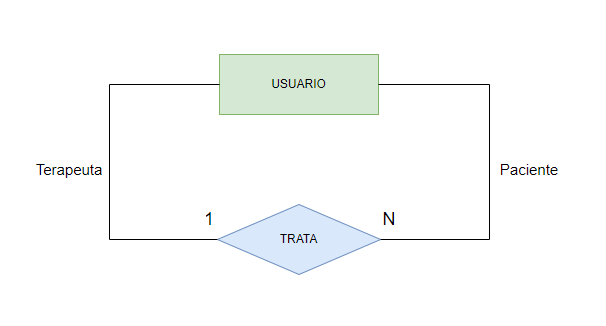
\includegraphics[scale=1.0]{Imagenes/Vectorial/diagrama_entidad_relacion_mysql}
	\caption{Diagrama de entidad-relación MySQL}
	\label{fig:diagramaEER}
\end{figure}

\subsection{Tabla de usuarios}
Es la tabla que alberga toda la información de los usuarios, tanto terapeutas como usuarios que se distinguirán mediante el campo ``type''.
Son los dos tipos de usuarios que podrán iniciar sesión en la aplicación. Por cada registro tendremos los campos que se muestran en la figura \ref{fig:diagramatablausers} y que se explican a continuación:

\begin{figure}[h]
	\centering
	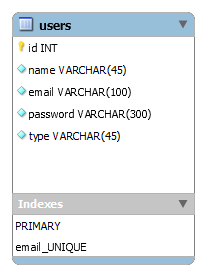
\includegraphics[scale=1.0]{Imagenes/Vectorial/diagrama_tabla_users}
	\caption{Diagrama de la tabla de usuarios}
	\label{fig:diagramatablausers}
\end{figure}

\begin{itemize}
	\item \textit{id}: El entero que representa el identificador de la fila, único y clave primaria para poder diferenciar cada registro inequívocamente
	\item \textit{name}: El nombre de usuario, una cadena de caracteres, que se utilizará para referirse al navegante en la aplicación web
	\item \textit{email}: El correo electrónico, una cadena de caracteres, único también para que no puedan existir dos usuarios con el mismo email, lo que supondría un error
	\item \textit{password}: La contraseña, cadena de caracteres que se guardará cifrada. Cuando se intente iniciar sesión, se comprobará si los datos son correctos y las contraseñas coinciden.
	\item \textit{type}: Cadena de caracteres que indica si el tipo de usuario es terapeuta o paciente. Es necesario distinguirles porque tendrán acceso a funcionalidades distintas en la aplicación web.
\end{itemize}

\subsection{Tabla de terapias}
Tabla en la que se guardan las relaciones entre terapeutas y sus pacientes. Por cada registro tenemos los campos que se muestran en la figura \ref{fig:diagramatablatherapy}. Las diferentes columnas de la tabla se explican a continuación:

\begin{figure}[h]
	\centering
	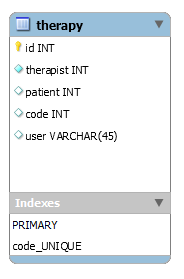
\includegraphics[scale=1.0]{Imagenes/Vectorial/diagrama_tabla_therapy}
	\caption{Diagrama de la tabla de terapias}
	\label{fig:diagramatablatherapy}
\end{figure}

\begin{itemize}
	\item \textit{id}: El entero que representa el identificador de la fila, único y clave primaria, se utiliza igual que en el de la tabla de usuarios.
	\item \textit{therapist}: El identificador del terapeuta al que le correponde la terapia  encargado de tratar al paciente que toque.
	\item \textit{patient}: El identificador del paciente señalado para la terapia
	\item \textit{code}: El entero que representa un código, único, para que el paciente pueda registrarse como tal en la aplicación y con su terapeuta asignado. Son números elegidos aleatoriamente del 100 al 999. Una vez se registra el paciente, no se vuelve a necesitar este código para nada.
	\item \textit{user}: Cadena de caracteres utilizada para identificar por nombre a un paciente que aún no se ha registrado pero sí tiene código asignado.
\end{itemize}


\section{Implementación final}

La aplicación final del chatbot, con la que el usuario con demencia interactuaría, se ha desarrollado usando el \textit{framework} de creación de aplicaciones ``Flask''. Se trata de un framework para la creación rápida de aplicaciones web desarrolladas con Python. Se estuvo planteando usar el framework ``Django'' pero finalmente se optó por Flask porque Django es para aplicaciones mucho más grandes y complejas de lo que se proponía crear para este trabajo. Flask es mucho más intuitivo y fácil de usar, además, con solo un par de líneas se puede levantar una aplicación web sin necesidad de librerías ni herramientas accesorias. Por otro lado, el diseño de la página web se ha desarrollado con hojas de estilos al uso, sin hacer uso de ningún framework para el frontend. Sin embargo, no se ha programado línea a línea sino que se ha replicado el estilo del sitio de administración\footnote{https://developer.mozilla.org/es/docs/Learn/Server-side/Django/Admin\_site} que proporciona ``Django'' a todos los desarrolladores de aplicaciones web que utilicen su framework. Como se había trabajado anteriormente con ``Django'', se ha querido utilizar su diseño visual por ser conocido y porque el objetivo de la aplicación era mostrar la usabilidad del chatbot, no que fuera visualmente bonito. No se ha trabajado con estilos más elaborados y técnicos para invertir ese tiempo en el desarrollo con Python.

Para empezar con Flask, se utilizó la guía\footnote{https://flask.palletsprojects.com/en/2.2.x/quickstart/} proporcionada por la página oficial de este framework y un tutorial\footnote{https://j2logo.com/leccion-1-la-primera-aplicacion-flask/} específico para la creación de aplicaciones como esta. Para empezar con Flask lo principal es tener instalado Python e instalar las dependencias necesarias del framework. Esto se puede hacer desde el propio entorno de desarrollo elegido, en mi caso ``Visual Studio Code'', usando el instalador de paquetes ``pip'' de Python. El paquete principal para que la aplicación funcione es el de Flask, en este caso Flask-WTF para que también incluya la validación de formularios, como sería el de inicio de sesión en el que se profundizará más adelante.  

Una vez instalados los paquetes, el despliegue de la aplicación es muy sencillo y, tan solo se necesitan unas pocas líneas de código para que funcione. Lo primero sería crear un fichero python, en nuestro caso llamado ``run.py'', en el que irán los métodos asociados a las URLs que formarán la aplicación, el primer método en nuestro caso, sería el que nos lleva a la página principal, el ``index'', que es básico para que funcione la aplicación. El fichero run.py más básico para que se despliegue la aplicación quedaría de esta forma:

\begin{verbatim}
	from flask import Flask
	app = Flask(__name__)
	
	@app.route('/')
	def index():
	return render_template("index.html")
\end{verbatim}

Para que tenga sentido este fichero sería necesario crear aparte un archivo HTML llamado ``index.html'' con la lógica de la página principal, que puede ser lo más sencilla que se quiera. Este código funcionará de tal forma que cuando se acceda a la url de la aplicación (identificada también por terminar con este símbolo ``/'') se va a cargar la página del index.html. Pero, antes, para arrancar la aplicación se necesita ejecutar varios comandos en el terminal:

\begin{verbatim}
	> $env:FLASK_APP = "run"
	> python -m flask run
\end{verbatim}

Flask incluye un servidor interno propio al que se podrá acceder desde \textit{localhost}. Para que este servidor sepa qué aplicación debe lanzar, se usa el primer comando que apunta al fichero run del directorio en el que se encuentra la aplicación. El segundo comando es el que definitivamente lanza la aplicación. Podemos comprobar que la aplicación funciona entrando a un navegador y accediendo a la URL ``http://127.0.0.1:5000/'' que cargará el fichero principal index.html. 

Una vez tenemos funcionando la aplicación ya solo queda ampliar sus funcionalidades que se explicarán a continuación. 


\subsection{Funcionalidad inicio de sesión y registro}

Se añade esta funcionalidad para que cada recuerdo se pueda asociar a un usuario y así dar la posibilidad de guardar incontables historias de vida de diferentes usuarios. De la mano del inicio de sesión, se encuentra la funcionalidad del registro de usuarios que se contará también en esta sección de la memoria. De nuevo, para ambas funcionalidades, se ha utilizado como guía el tutorial de Flask\footnote{https://j2logo.com/tutorial-flask-leccion-3-formularios-wtforms/} de la página ``J2logo''. En este caso, la página web nos guía en el uso de formularios en Flask, que se requieren tanto para el inicio de sesión como para el registro de usuarios. 

%Los formularios que se necesiten para una aplicación de Flask es conveniente tenerlos separados en un archivo Pyhton aparte, en este caso en ``forms.py''. En este archivo se definirán las clases SignUpForm y LoginForm que heredan de la clase FlaskForm. Dentro de estas clases se definirán los atributos, variables que se corresponden con los campos a validar del formulario. La validación de los campos se hará automáticamente teniendo en cuenta el tipo de dato que se defina para cada atributo y también los parámetros opcionales que se definan para ese atributo. Por ejemplo, para el campo del email que se usa en ambos formularios se define el siguiente atributo:

%\begin{verbatim}
%	email = StringField('Email', validators=[DataRequired(), Email()])
%\end{verbatim}

%Este atributo \textit{email} se ha definido como una cadena de caracteres y como parámetros opcionales tiene ``DataRequired(), Email()''. Es decir, cuando se haga la validación del formulario, la aplicación comprobará que el campo no está vacío y que en efecto, se trata de un correo electrónico basándose en su formato. 

%Aparte de haber definido el formulario, se necesita una url asociada a cada página, tanto la de inicio de sesión como la de registro. Como había comentado antes, las URLs que formen parte de la aplicación deben estar definidas en el fichero ``run.py''. Serán respectivamente las URLs ``/login'' y ``/signup''. Hay dos funciones, una para gestionar el inicio de sesión y otra para el registro. Ambas funciones usan los métodos \textit{GET} y \textit{POST} porque necesitan enviar datos a la página web y recibirlos también. En estas funciones, además, será donde se invoque a las clases que se crearon anteriormente de los formularios, creando una instancia de las mismas.


Para iniciar sesión en la aplicación (ver Figura \ref{fig:funcionalidadlogin}), tanto terapeutas como pacientes deben introducir los campos email y contraseña que se hayan usado en el registro. Si existe en la base de datos un usuario cuyo email coincide con el introducido y, además, la contraseña es correcta se dará acceso al usuario al resto de funcionalidades y se le redirigirá de nuevo a la página principal pero ya identificado.En el caso de que el email no exista o la contraseña sea incorrecta se mostrará el siguiente error: ``Error al iniciar sesión'', y se pedirán los datos de nuevo.

\begin{figure}[h]
	\centering
	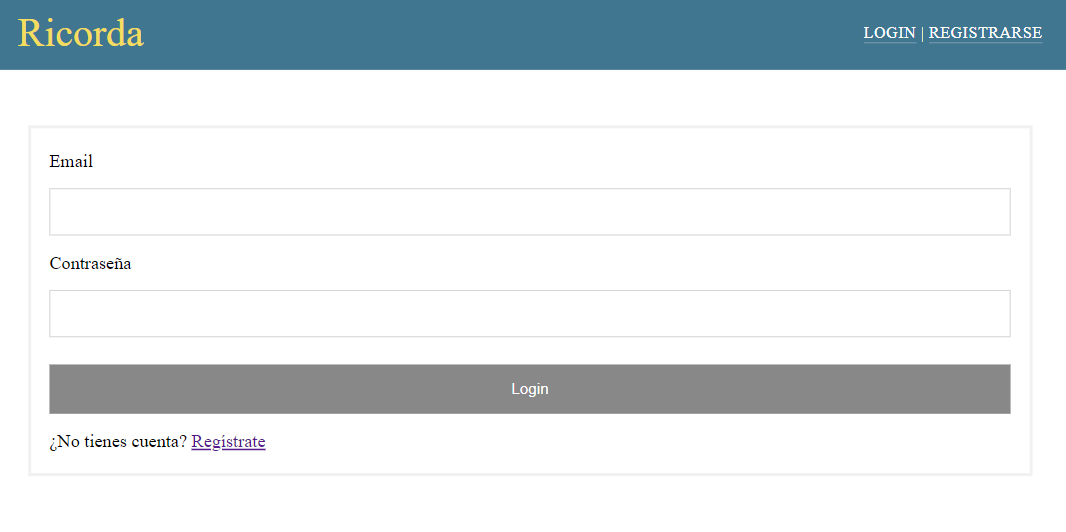
\includegraphics[scale=0.7]{Imagenes/Vectorial/funcionalidad_login1}
	\caption{Funcionalidad inicio de sesión}
	\label{fig:funcionalidadlogin}
\end{figure}

La página de registro (ver Figura \ref{fig:funcionalidadsignin}) es parecida a la de inicio de sesión pero añadiendo varios campos más a rellenar. El primero es el del nombre, que se utilizará para que la aplicación se dirija al usuario por ese nombre. El email y la contraseña se guardarán en la base de datos de MySQL y se utilizarán para comprobar si el inicio de sesión es correcto. La contraseña se guarda encriptada mediante un hash gracias a la librería ``werkzeug.security'' de Python, que proporciona funciones para generar el \textit{hash} y para comprobar si una cadena de caracteres dada coincide con la contraseña encriptada. Después, hay que rellenar el campo ``Tipo'' que indica a la aplicación si el usuario que se registra lo hará como terapeuta o como paciente. En el caso de registrarse un paciente, su terapeuta asociado y ya registrado, le debe haber proporcionado un código que introducirá en el campo ``Código''. Esto es necesario para que el usuario se reconozca como paciente del terapeuta correspondiente porque sino el terapeuta no puede acceder a la información del usuario. Una vez registrado el paciente, se crea un nuevo registro que le aparece al terapeuta en el listado de pacientes (ver Figura \ref{fig:funcionalidadconsultadepacientes}) y a partir de ese momento, podrá consultar toda su información. En caso de introducir un código erróneo se muestra el siguiente error: ``Error: No existe terapia para ese código''. A nivel backend, el código introducido debe haberse registrado anteriormente en la tabla de terapias y asociado al terapeuta que lo creó. En caso de registrarse un terapeuta, el valor del código no es relevante. Si el email proporcionado ya está registrado por otro usuario, se muestra el siguiente error: ``Error: El email ya está siendo utilizado por otro usuario'', y se pedirán los datos de nuevo.

\begin{figure}[h]
	\centering
	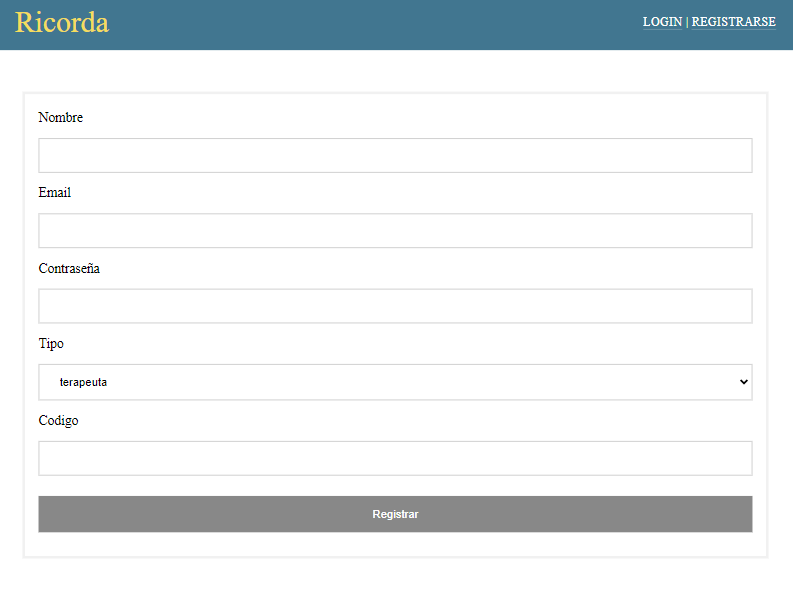
\includegraphics[scale=0.6]{Imagenes/Vectorial/funcionalidad_signin1 }
	\caption{Funcionalidad registro}
	\label{fig:funcionalidadsignin}
\end{figure}

\subsection{Funcionalidad chatbot}

El chatbot (ver Figura \ref{fig:funcionalidadchatbot}) es la funcionalidad principal de la aplicación y es en lo que a nivel de backend se ha invertido más tiempo. Sin la parte visual del frontend, el chatbot también funciona desde la línea de comandos de Python. Sin embargo, se ha decidido hacer la aplicación web para facilitar la interacción con el usuario. Esta funcionalidad permitirá al usuario interactuar con el bot que hay detrás a través de un chat. Se distingue de otras inteligencias artificiales de tipo chatbot porque es el bot quien dirige la conversación y el que pregunta o habla con el usuario y no al revés. Por ejemplo, el usuario es el que hace peticiones a Alexa que interpreta lo que ha dicho el usuario y le ofrece un servicio. Sin embargo, el chatbot ``Ricorda'' es el que guía la conversación.

En primer lugar, el bot saluda al usuario, le da la bienvenida y explica que comenzará a hacer preguntas. La primera pregunta se escoge al azar de entre los documentos almacenados en la colección de preguntas. Además, se filtran aquellos que contengan preguntas que ya hayan sido preguntadas al usuario en cuestión. Dada la primera pregunta, se espera a que el usuario responda, solo podrá mandar un único mensaje por cada pregunta porque está configurado de tal forma que responde tras procesar solo un mensaje. La respuesta del usuario se trata y almacena como se explica en el capítulo de la arquitectura del chatbot, es decir, se clasifica según la etapa de vida a la que corresponde (infancia, juventud, etapa adulta y vejez), se clasifica en positivo o negativo con el analizador de sentimientos del texto, se almacena en la colección de respuestas de la base de datos de mongo junto al id del usuario, la pregunta y las categorías anteriores y, finalmente, se le somete a un análisis léxico para conseguir la mejor siguiente pregunta, la que mayor relación encuentre con la respuesta que ha dado el usuario. Después del análisis de la respuesta del usuario, se lanza la siguiente pregunta aquella que más se corresponda con la respuesta del usuario. La persona volvería a responder y el bot a preguntar hasta que se canse de contestar a las preguntas. Todas las respuestas se almacenan y van así formando la historia de vida del paciente, recuerdo a recuerdo. Estos recuerdos se podrán consultar en la propia página web clasificados en etapas de vida, funcionalidad que se explica más adelante.

\begin{figure}[h]
	\centering
	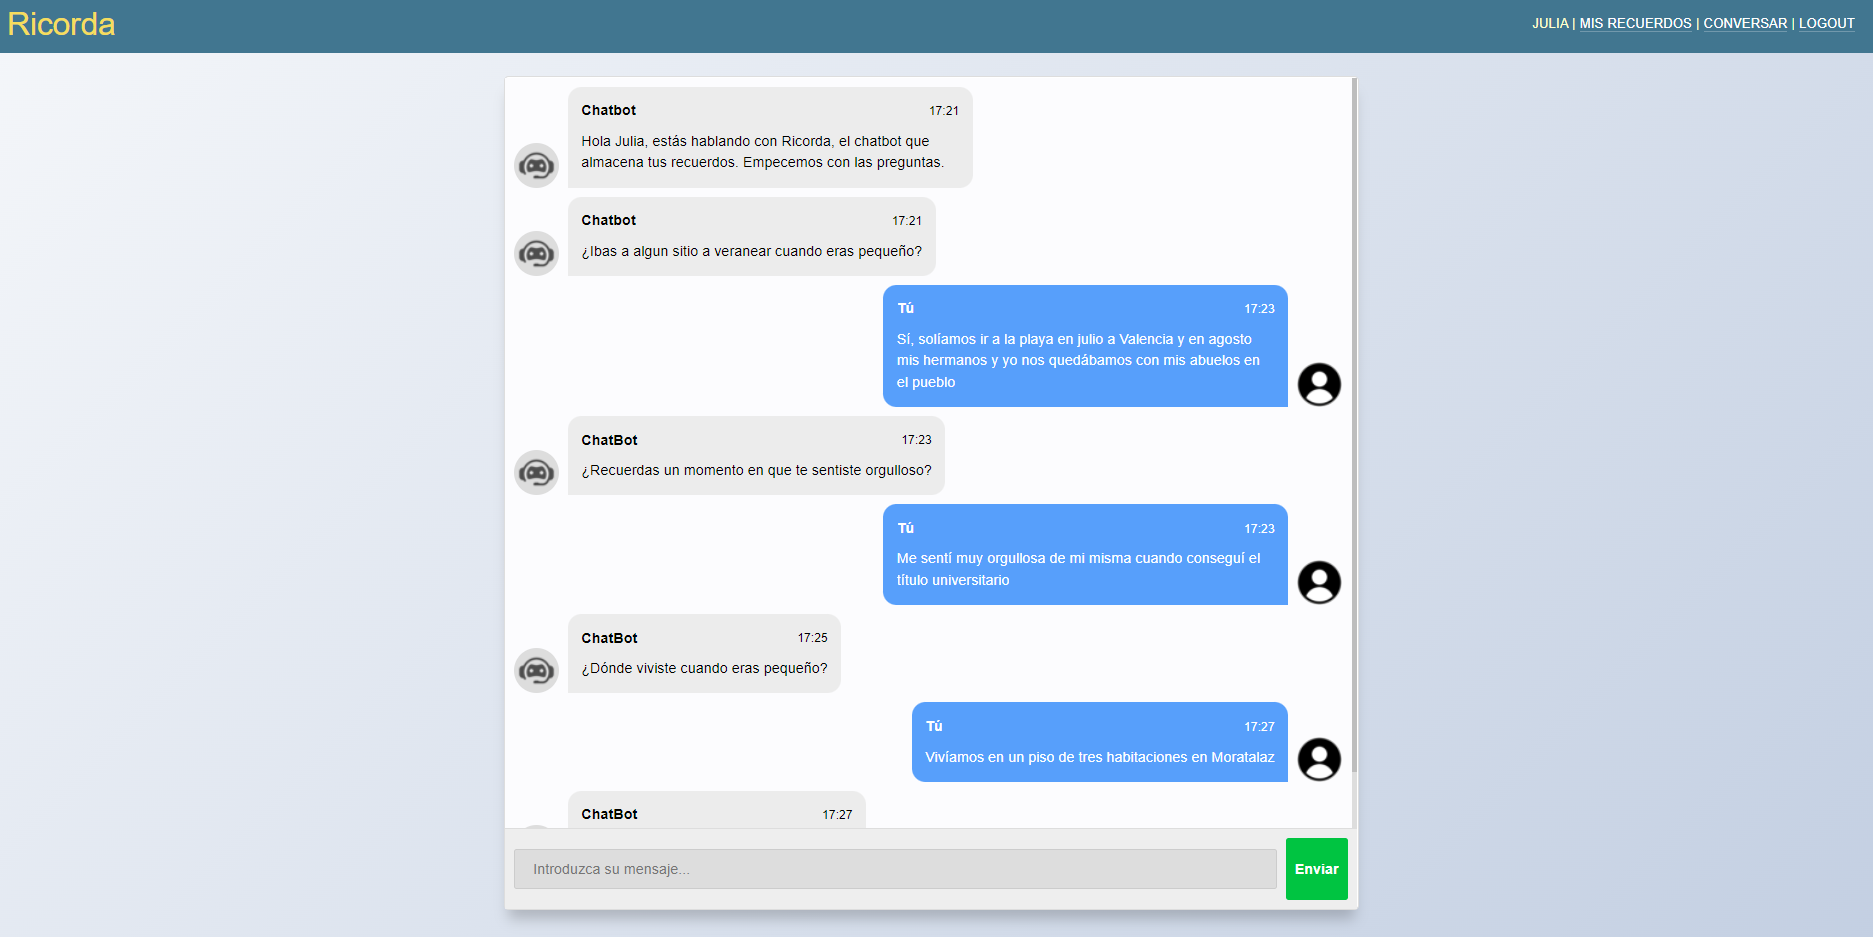
\includegraphics[scale=0.4]{Imagenes/Vectorial/funcionalidad_chatbot}
	\caption{Funcionalidad chatbot}
	\label{fig:funcionalidadchatbot}
\end{figure}

El diseño de esta vista esta inspirado en el Chatbot web de la página sobre inteligencia artificial ``Buff ML''\footnote{https://buffml.com/web-based-chatbot-using-flask-api/}

\subsection{Funcionalidad usuario terapeuta vs usuario paciente}

Dentro de la aplicación existen dos roles para los usuarios, el terapeuta podrá acceder al listado de sus pacientes y a los recuerdos ya recogidos por el chatbot. Por otro lado, el paciente podrá acceder al chatbot con el que interactuará para sacar el mayor número de recuerdos y también consultar toda la información guardada sobre él y sus respuestas.

Los usuarios pacientes podrán acceder a un menú concreto pensado para que puedan acceder a las funcionalidades que les interesan. El menú de los pacientes se puede ver en la Figura \ref{fig:funcionalidad_terapeutavspaciente2}. El menú para los usuarios terapeutas es distinto y está pensado para que puedan acceder directamente a las funcionalidades que les corresponden. Se puede ver en la Figura \ref{fig:funcionalidadterapeutavspacientes}. Estos menús siempre están disponibles en la esquina superior derecha de la página.

\begin{figure}[h]
	\centering
	
\includegraphics[scale=1.0]{Imagenes/Vectorial/funcionalidad_terapeutavspaciente2}
	\caption{Menú de los pacientes}
	\label{fig:funcionalidad_terapeutavspaciente2}
\end{figure}

\begin{figure}[h]
	\centering
	
\includegraphics[scale=1.0]{Imagenes/Vectorial/funcionalidad_terapeutavspaciente}
	\caption{Menú de los terapeutas}
	\label{fig:funcionalidadterapeutavspacientes}
\end{figure}

\subsection{Funcionalidad consulta de pacientes registrados por parte del terapeuta}

Un terapeuta debe tener la posibilidad de ver una lista de pacientes que estén a su cargo y a los que trata en terapias. Esta funcionalidad está disponible en el apartado ``pacientes'' del menú (ver Figura \ref{fig:funcionalidadconsultadepacientes}). En esta página tendrá acceso a una tabla con todos sus pacientes que tiene dos columnas, la primera indica el nombre con el que están registrados los pacientes y, la segunda muestra el email asociado a cada uno. Si lo que quiere es obtener la información de uno de sus pacientes, es decir, los recuerdos que ha ido introduciendo el usuario y recogiendo el chatbot divididos por etapas vitales, se puede ver pulsando en la fila correspondiente, concretamente, en el enlace que hay en el nombre de esa persona. Será así redirigido a la página de historia de vida de un paciente. Encima de la tabla de pacientes, en la esquina superior derecha de la página también hay un botón que dice ``Nuevo paciente'' con el que se accede a la página de creación de un nuevo paciente. Se trata de una funcionalidad para registrar a un nuevo usuario asociado al terapeuta para que pueda tener acceso a la aplicación y por ende, al chatbot.

\begin{figure}[h]
	\centering
	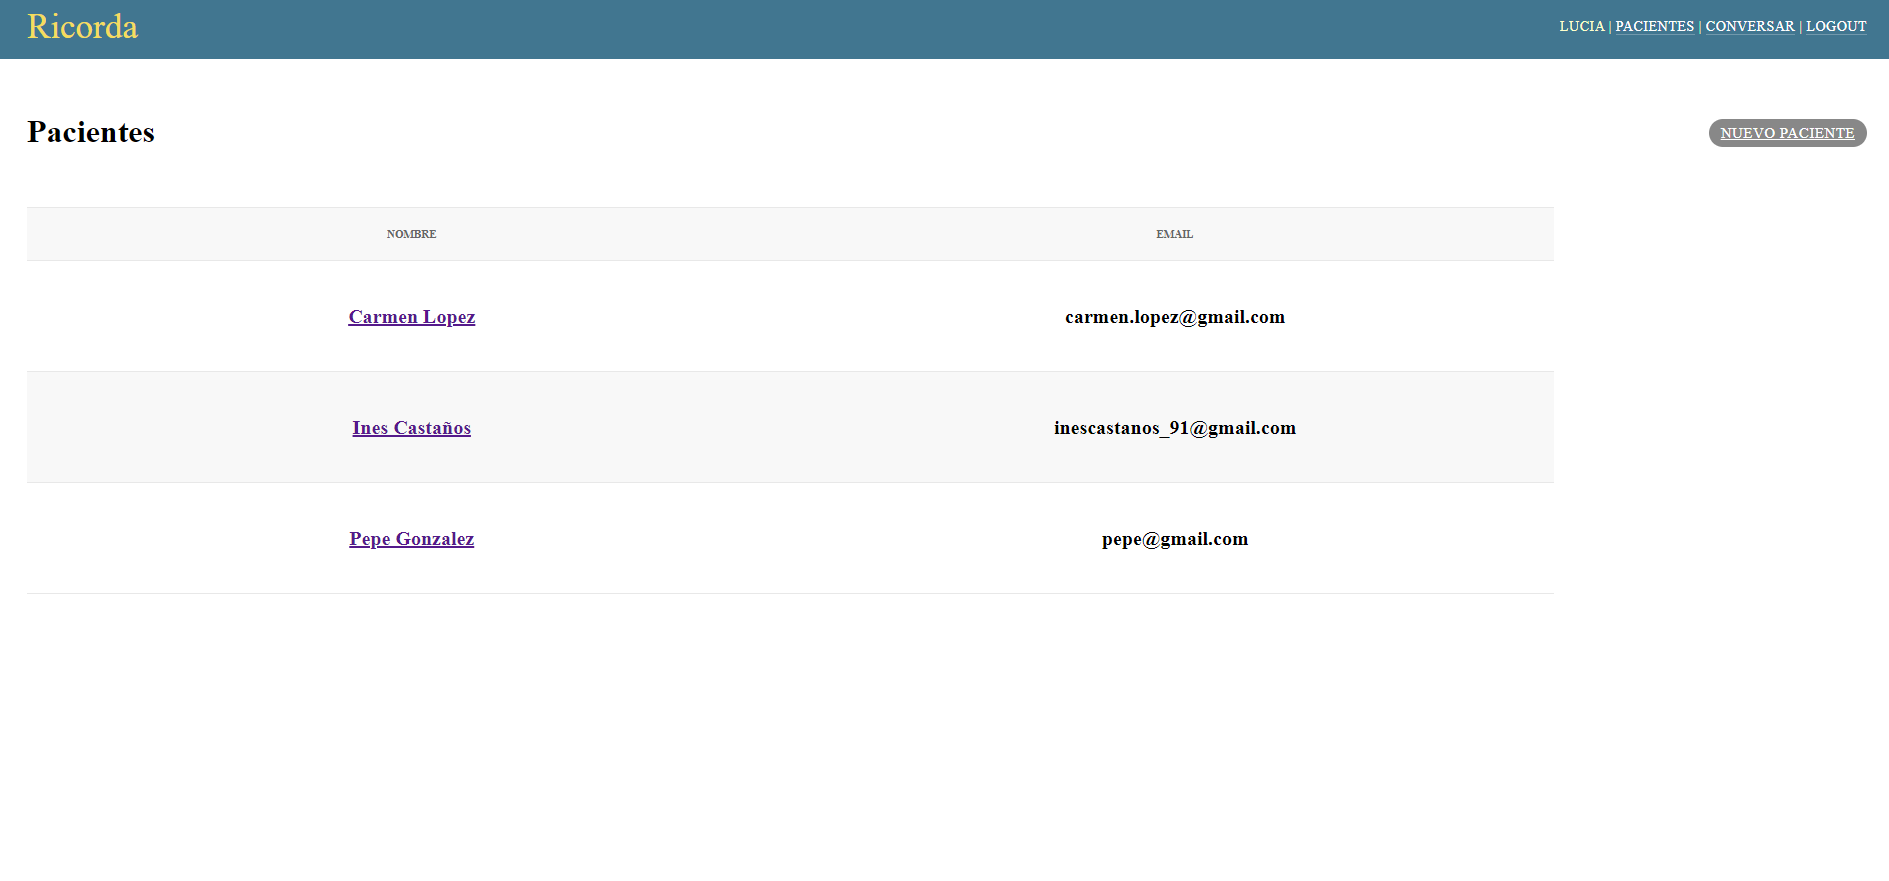
\includegraphics[scale=0.3]{Imagenes/Vectorial/funcionalidad_consultar_pacientes}
	\caption{Funcionalidad consultar pacientes registrados}
	\label{fig:funcionalidadconsultadepacientes}
\end{figure}

\subsection{Funcionalidad crear nuevo paciente}

Se trata de una funcionalidad exclusiva del terapeuta. Desde la página del listado de pacientes se accede a la página de creación de un nuevo paciente clicando el botón de la esquina superior derecha ``NUEVO PACIENTE''. Una vez pulsado se muestra algo parecido a lo reflejado en la Figura \ref{fig:funcionalidadnuevopaciente}, por un lado, en la parte de arriba se encuentra un formulario para registrar a un paciente. Hay dos datos claves, el nombre, que debe rellenarlo el terapeuta, y el código, un número aleatorio, por seguridad, del 100 al 999 (a priori no se necesita un rango mayor) que viene dado por el programa y que no ha sido utilizado antes para otro usuario. El código es necesario para que el paciente pueda registrarse en la página de registro de usuarios y es tarea del terapeuta comunicárselo para que ambos usuarios estén conectados gracias a la tabla de terapias. El nombre se introduce para que el terapeuta pueda reconocer el código fácilmente gracias a estar etiquetado. Esto es importante para la segunda parte de la página, la que se encuentra debajo del formulario. El terapeuta va a tener siempre acceso a los códigos que ya ha registrado. Es decir, se muestra una tabla con dos columnas, la del usuario y la del código. La del usuario se corresponde con el campo ``nombre'' del formulario y la del código muestra el número que debe introducir el paciente para poder registrarse. Cuando el paciente se registra con su código, la fila correspondiente se elimina de la tabla de usuarios sin registrar y, así, el terapeuta puede tener un control de los usuarios dados de alta en la aplicación, a los que puede ir haciendo un seguimiento. También puede controlar los usuarios que todavía faltan por registrar, a los que a lo mejor es necesario recordar el código. 

A nivel base de datos, cuando se valida este formulario del código, se añade un registro en la tabla de terapias de la base de datos MySQL con los siguientes cinco campos: 
\begin{itemize}
	\item Id de la terapia, clave primaria
	\item Id del terapeuta al que estará asociado el paciente
	\item Id del paciente, inicializado a ``null'' porque no existirá ese usuario en la tabla de usuarios hasta que no se registre
	\item Código
	\item Nombre con el que se asocia el código.
\end{itemize}

Cuando el paciente se registre en la aplicación, en el campo de id del paciente se introducirá el id del nuevo usuario. Además, tanto el campo de código como el de nombre se pondrán a ``null'' porque ya no son necesarios. El número del código se puede reutilizar. En la Figura \ref{fig:funcionalidadnuevopacientetablaterapias} se puede ver que el único usuario no registrado para el terapeuta con id ``1'' es el de Mario. El resto de terapias tienen los ids de ambos usuarios rellenos. El registro con id ``9'' de la tabla de terapias es el que sale en la tabla de la parte inferior de la página de la Figura \ref{fig:funcionalidadnuevopaciente} porque es el único sin registrar.  
 
 \begin{figure}[h]
 	\centering
 	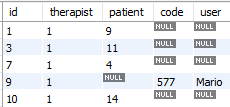
\includegraphics[scale=1.6]{Imagenes/Vectorial/funcionalidad_nuevo_paciente_tabla_terapias}
 	\caption{Tabla de terapias en MySQL}
 	\label{fig:funcionalidadnuevopacientetablaterapias}
 \end{figure}

\begin{figure}[h]
	\centering
	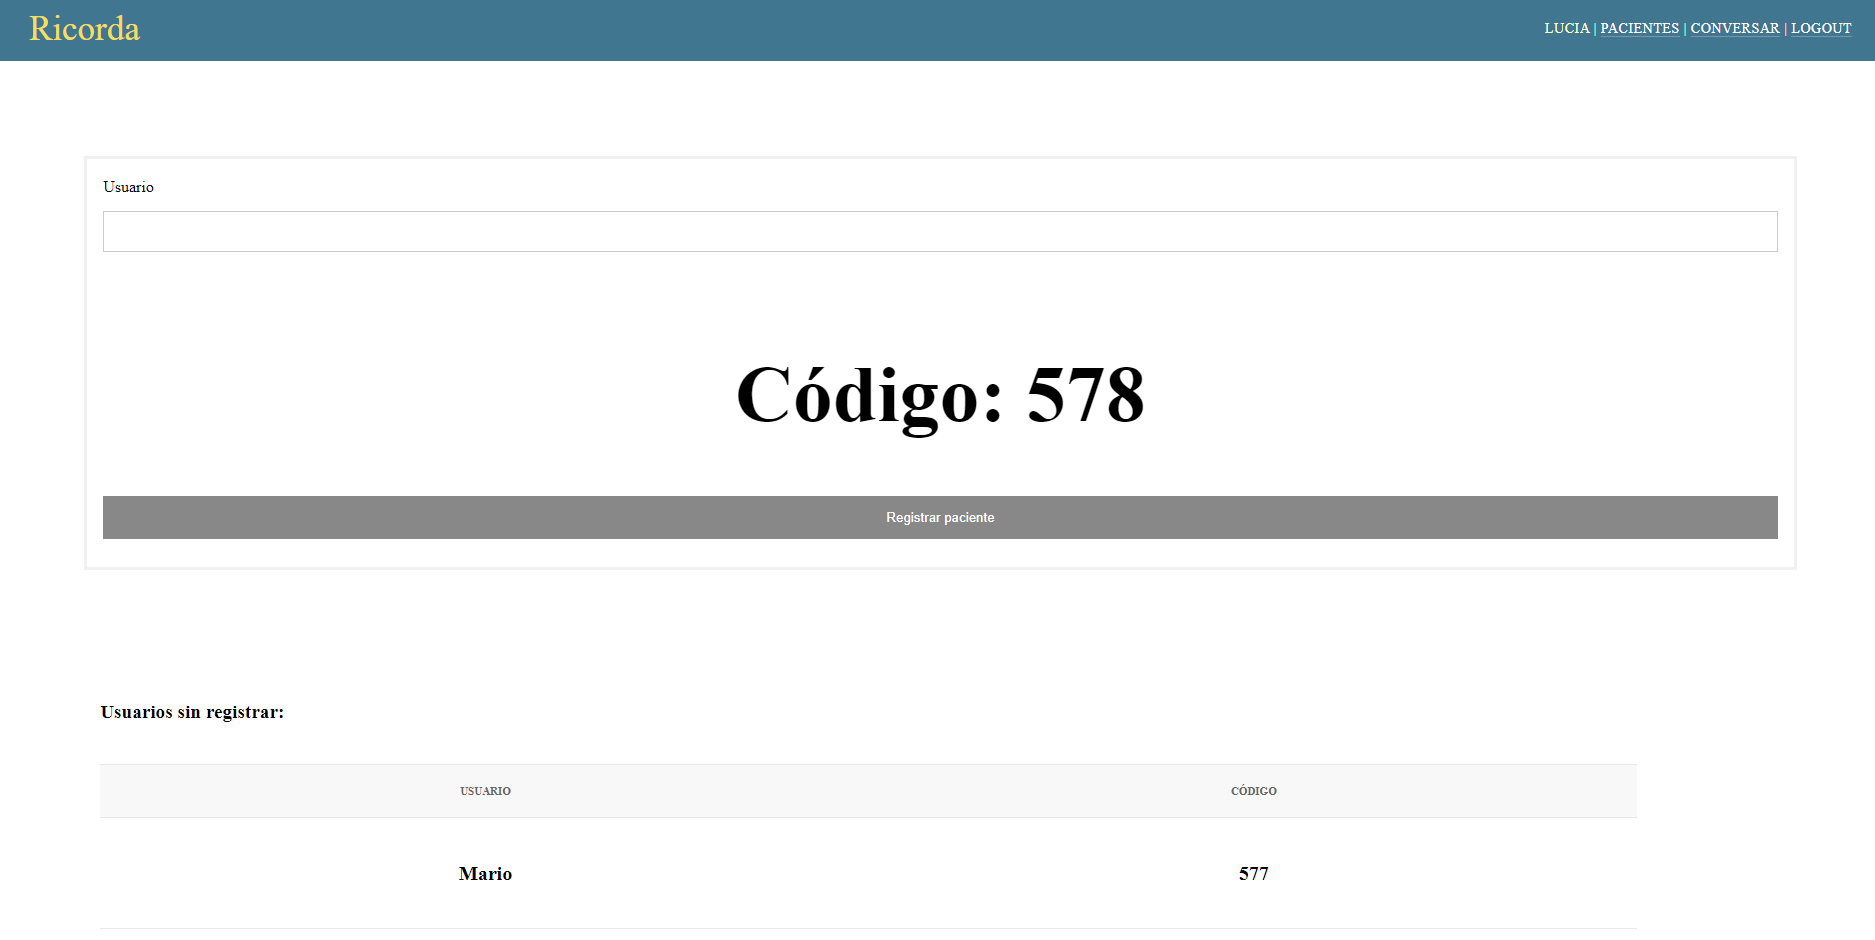
\includegraphics[scale=0.3]{Imagenes/Vectorial/funcionalidad_nuevo_paciente}
	\caption{Funcionalidad crear nuevo paciente}
	\label{fig:funcionalidadnuevopaciente}
\end{figure}


\subsection{Funcionalidad recopilación de los recuerdos de un paciente}

Los recuerdos que se van almacenando para cada usuario en la base de datos se van a poder consultar en esta vista (ver Figura \ref{fig:funcionalidadhistoriavida}). La historia de vida de una persona se va construyendo desde su infancia hasta los últimos años de vida. Esta progresión es lo que pretende reflejar esta funcionalidad. Empezando con la infancia y terminando por la vejez, se muestran los recuerdos del usuario clasificados en cuatro etapas: infancia, juventud, etapa adulta y vejez. Esta categorización se obtiene de la base de datos de Mongo, en concreto de la tabla de respuestas que da el usuario al chatbot. Antes de ser almacenados en la base de datos, los recuerdos se analizan con el clasificador de etapas y sentimientos (explicado en el capítulo de arquitectura del chatbot) y, luego, se guardan junto a las categorías. En esta vista, para cada etapa se enumeran los recuerdos (respuestas al chatbot) correspondientes junto a la pregunta que se le hizo al usuario. Si alguna de las cuatro etapas no tiene recuerdos asociados, no se muestra el apartado. 

\begin{figure}[h]
	\centering
	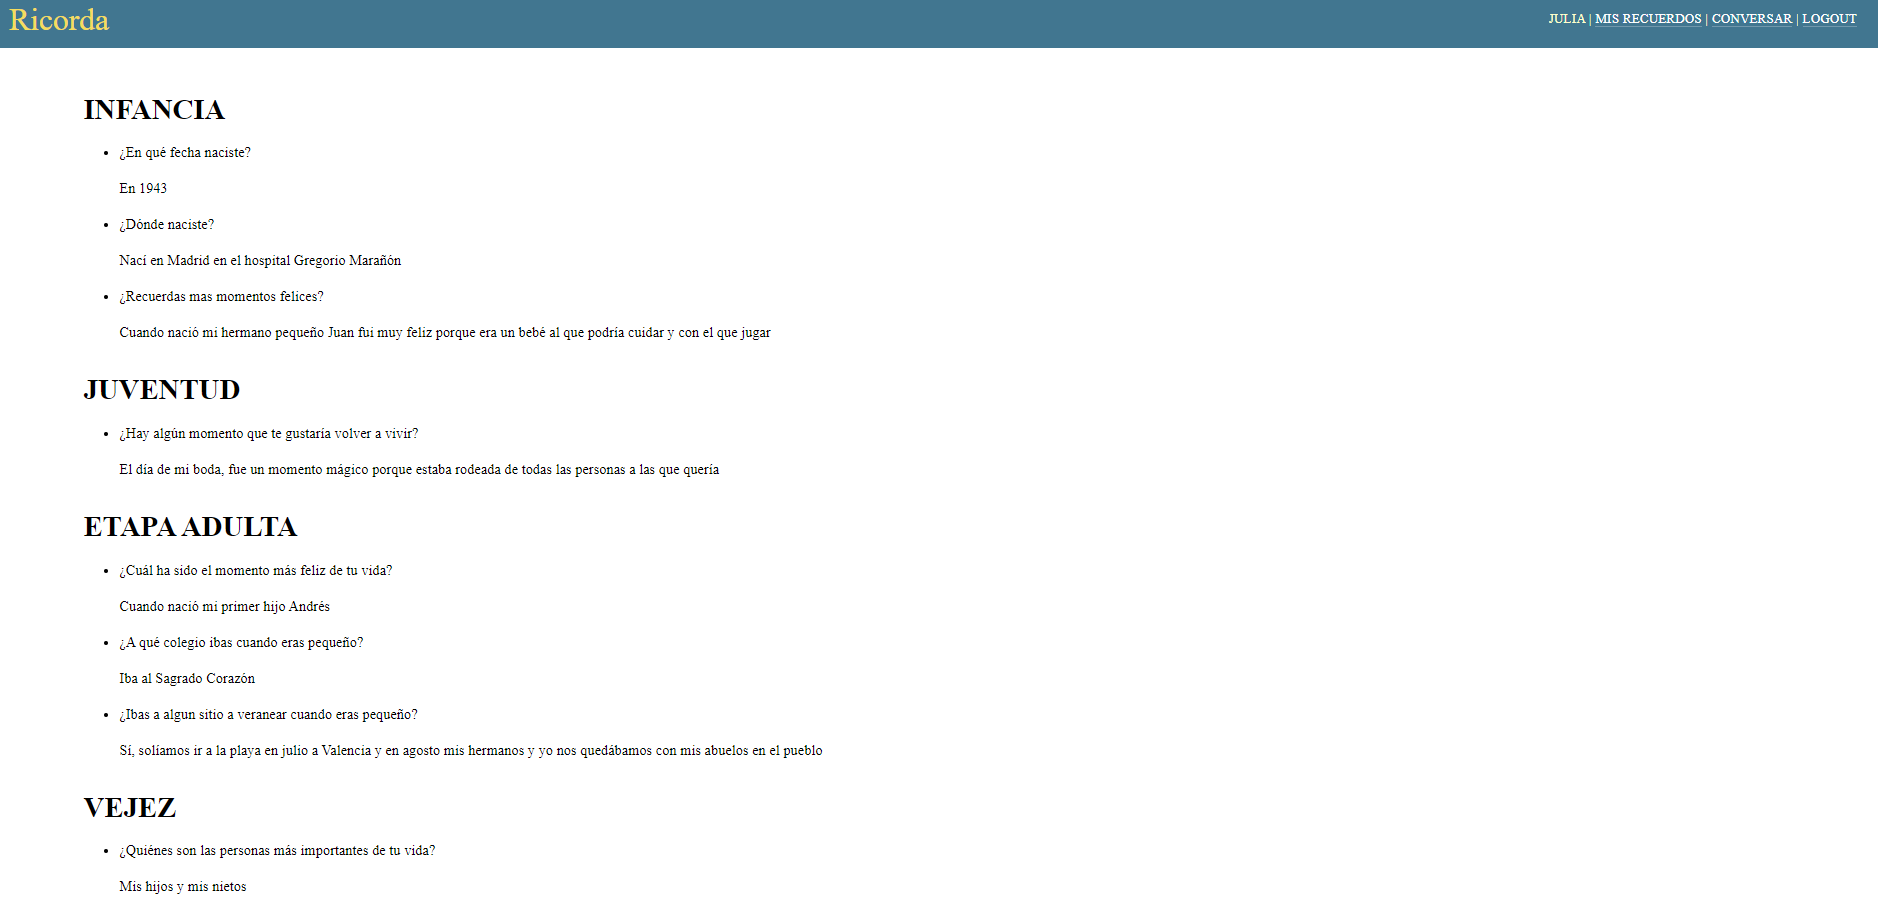
\includegraphics[scale=0.45]{Imagenes/Vectorial/funcionalidad_historia_vida}
	\caption{Funcionalidad recopilación de recuerdos del paciente}
	\label{fig:funcionalidadhistoriavida}
\end{figure}




